%------------------------------------------------
% Introduction.tex
%
% This document build the introduction frame
%------------------------------------------------
\section{Nuova funzione di Service Desk}
\frame
{
\frametitle{Contenuti}
\tableofcontents[currentsection]
%\addtocounter{framenumber}{-1}
}

\subsection*{Introduzione}
\begin{frame}{Introduzione \small{1/3}}
L'ente proponente intende proporre all'amministrazione dell'ospedale G. Pini l'implementazione della funzionalità di
\begin{figure}

\includegraphics[scale=0.3]{Images/Service_desk.png}
\end{figure}
in quanto si vuole:
\begin{itemize}
\item{la gestione di \textbf{servizi IT}}
\item{offrire un servizio di \textbf{qualità}}
\item{avere un unico Service Point Of Contact (SPOC)}
\item{avere uno strumento per valutare il livello generale di ``salute''}
\end{itemize}
\end{frame}

\begin{frame}{Introduzione \small{2/3}}
\begin{columns}
\begin{column}{0.75\textwidth}
Benefici voluti nella struttura ospedaliera:
\begin{itemize}
\item{incremento soddisfazione degli utenti}
\item{maggior accessibilità all'assistenza}
\item{miglior qualità nelle risposte}
\item{maggior lavoro di gruppo}
\item{approccio proattivo}
\end{itemize}
\end{column}
\begin{column}{0.25\textwidth}
\begin{figure}

\includegraphics[scale=0.5]{Images/Benefit.png}
\end{figure}
\end{column}
\end{columns}
\end{frame}

\begin{frame}{Introduzione \small{3/3}}
\begin{theorem}[Obiettivo]
L'obiettivo primario del nuovo Service Desk consiste nel ripristinare i normali livelli di servizio agli utenti, il più velocemente possibile, a seguito di incidenti.
\end{theorem}
\begin{columns}
\begin{column}{0.8\textwidth}
``ripristino dei normali livelli di servizio'' inteso come:
\begin{itemize}
\item{risoluzione di incidenti}
\item{soddisfazione delle richieste degli utenti}
\item{fornire risposta alle loro domande}
\end{itemize}
\end{column}
\begin{column}{0.2\textwidth}
\begin{figure}
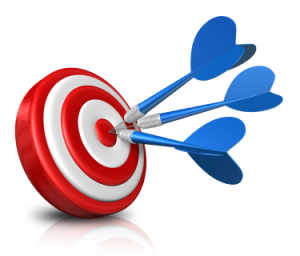
\includegraphics[scale=0.25]{Images/Objectives.png}
\end{figure}
\end{column}
\end{columns}
\end{frame}

\subsection*{Risorse e budget}
\begin{frame}{Risorse possedute}
L'ospedale G. Pini dispone di un elevato numero di risorse:
\begin{itemize}
\item{\textit{hardware}}
\item{\textit{software}}
\item{infrastruttura tecnologica}
\item{contratti attivi}
\end{itemize}
\vspace{5mm}
\begin{columns}
\begin{column}{0.7\textwidth}
per cui il personale del SD verrà suddiviso in personale a supporto:
\begin{itemize}
\item{dell'area amministrativa}
\item{dell'area sanitaria}
\item{dell'infrastruttura}
\end{itemize}
\end{column}
\begin{column}{0.3\textwidth}
\begin{figure}

\includegraphics[scale=0.15]{Images/Categories.png}
\end{figure}
\end{column}
\end{columns}
\end{frame}

\begin{frame}{Costi \small{1/2}}
Budget iniziale di: \textbf{1500000.00} \euro{}
\begin{table}
\begin{tabular}{ l | r | c | c | r }
\textbf{Descrizione} & \textbf{Costo} & \textbf{Quantità} & \textbf{Mensilità} & \textbf{Totale}\\
\hline
\hline
\textsc{installazione} & 5000.00 \euro{} & 1 & 1 & 5000.00 \euro{}\\
\textsc{licenza} & 110.00 \euro{} & 31 & 12 & 40920.00 \euro{}\\
\textsc{manutenzione} & 1000.00 \euro{} & 1 & 1 & 1000.00 \euro{}\\
\textsc{formazione} & 1000.00 \euro{} & 15 giorni & 1 & 15000.00 \euro{}\\
& & & \textbf{TOTALE} & \textbf{61920.00 \euro{}}\\
\end{tabular}
\caption{Costi di implementazione primo anno}
\end{table}
\end{frame}

\begin{frame}{Costi \small{2/2}}
\begin{table}
\begin{tabular}{ l | r  }
\textbf{Anno} & \textbf{Costo}\\
\hline
\hline
\textsc{I anno} & 61920.00 \euro{}\\
\textsc{II anno} & 41920.00 \euro{}\\
\textsc{III anno} & 41920.00 \euro{}\\
\textsc{IV anno} & 41920.00 \euro{}\\
\textsc{V anno} & 41920.00 \euro{}\\
\textbf{TOTALE} & \textbf{229600.00 \euro{}}\\
\end{tabular}
\caption{Costi di implementazione anni successivi}
\end{table}
\end{frame}

\subsection*{Ruoli e responsabilità}
\begin{frame}{Ruoli e responsabilità}
All'interno del Service Desk sono stati individuati i seguenti ruoli:
\begin{itemize}
\item{Service Desk Manager}
\item{Service Desk Supervisior}
\item{Service Desk Analyst}
\end{itemize}
\begin{columns}
\begin{column}{0.4\textwidth}
\end{column}
\begin{column}{0.6\textwidth}
\begin{figure}
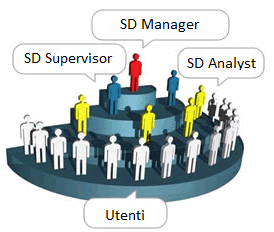
\includegraphics[scale=0.6]{Images/Roles.png}
\end{figure}
\end{column}
\end{columns}
\end{frame}

\subsection*{Struttura scelta}
\begin{frame}{Struttura scelta}
\begin{columns}
\begin{column}{0.6\textwidth}
SD di tipo \textbf{centralizzato} perché:
\begin{itemize}
\item{dimensioni ridotte della struttura}
\item{miglior gestione delle risorse}
\item{posizione geografica}
\end{itemize}
\end{column}
\begin{column}{0.4\textwidth}
\hspace{10mm}
\centering
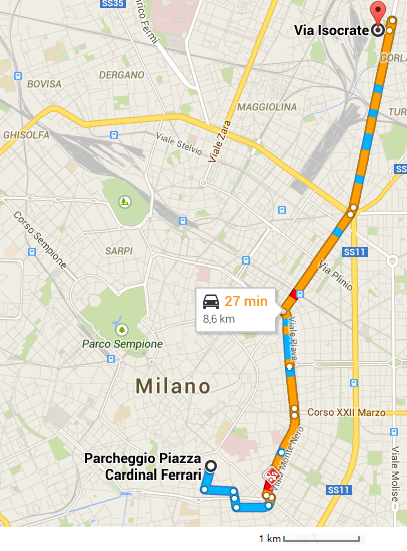
\includegraphics[scale=0.4]{Images/Maps.png}
\end{column}
\end{columns}
\end{frame}

\subsection*{User Experience}
\begin{frame}{User Experience}
Interventi da effettuare per una migliore User Experience:
\begin{itemize}
\item{garantire accessibilità alle informazioni}
\item{fornire canali di comunicazione}
\item{fornire materiale necessario:}
\begin{itemize}
\item{software SaaS}
\item{portale utente}
\item{desktop remoto}
\end{itemize}
\end{itemize}
\end{frame}

\subsection*{Operatività e contatti}
\begin{frame}{Operatività e contatti}
I tempi di operatività sono stati studiati tenendo conto:
\begin{itemize}
\item{orario di utilizzo di ogni servizio IT}
\item{carico di lavoro ospedaliero (statistiche)}
\end{itemize}
\begin{columns}
\begin{column}{0.7\textwidth}
Sarà contattabile attraverso:
\begin{itemize}
\item{portale web}
\item{e-mails}
\item{contatto telefonico}
\end{itemize}
\end{column}
\begin{column}{0.3\textwidth}
\begin{figure}

\includegraphics[scale=0.2]{Images/Contact.png}
\end{figure}
\end{column}
\end{columns}
\end{frame}

\subsection*{Samanage}
\begin{frame}{Samanage}
Il software \textbf{samanage} permette:
\begin{columns}
\begin{column}{0.8\textwidth}
\begin{itemize}
\item{gestione attività a supporto del SD}
\item{gestione di contratti e licenze}
\item{gestione KB e portale self-service}
\item{gestione ed analisi report}
\item{integrazione con Active Directory}
\item{gestione assets}
\item{gestione anomalie}
\item{gestione problemi e cambiamenti}
\item{gestione Service Catalogue}
\item{gsetione documenti SLM}
\end{itemize}
\end{column}
\begin{column}{0.2\textwidth}
\begin{figure}
\hspace{-20mm}
\vspace{20mm}

\includegraphics[scale=0.4]{Images/Samanage.png}
\end{figure}
\end{column}
\end{columns}
\end{frame}